\documentclass[12pt]{report}
\usepackage[fontsize=13pt]{scrextend}
\usepackage[utf8]{vietnam}
\usepackage[utf8]{inputenc}
\usepackage[vietnamese]{babel}
\usepackage{titlesec}
\usepackage{titletoc}
\usepackage{listings}
\usepackage[bookmarks=true]{hyperref}
\usepackage[left=3cm,right=2cm,top=2.5cm,bottom=3cm]{geometry}
\usepackage{graphicx}
\usepackage{hyperref}
\usepackage{tikz}
\usepackage{varwidth}
\usepackage{float}
\usepackage{listings}
\usepackage{color}
\usepackage{multirow}
\usepackage{booktabs}
\usepackage[ruled,vlined]{algorithm2e}
\usepackage{chngcntr}
\usepackage{nameref}
%\usepackage[font=bf]{caption}
%\counterwithin{figure}{chapter}

\renewcommand\labelitemi{--}

\setlength{\parskip}{6pt}

\usetikzlibrary{calc}
\setlength{\parindent}{10mm}
\renewcommand{\baselinestretch}{1.3}
\graphicspath{{images/}}

%%% The following lines add Chapter or Appendix in front of the number
\titlecontents{chapter}%
[0pt]%
{\vspace{1ex}}%
{\bfseries Chương \thecontentslabel\quad}%
{\bfseries}%
{\bfseries\hfill\contentspage}
%%% Initially, for the main part of the document, set the label to "Chapter"
\let\chapappname\chaptername

\definecolor{dkgreen}{rgb}{0,0.6,0}
\definecolor{gray}{rgb}{0.5,0.5,0.5}
\definecolor{mauve}{rgb}{0.58,0,0.82}

% setup code area as listings
\lstset{frame=tb,
  language=Java,
  aboveskip=3mm,
  belowskip=3mm,
  showstringspaces=false,
  columns=flexible,
  basicstyle={\small\ttfamily},
  numbers=left,
  numberstyle=\tiny\color{gray},
  keywordstyle=\color{blue},
  commentstyle=\color{dkgreen},
  stringstyle=\color{mauve},
  breaklines=true,
  breakatwhitespace=true,
  tabsize=3
}

\renewcommand{\lstlistingname}{Mã nguồn}

\newenvironment{thuattoan}[1][h]
  {\renewcommand{\algorithmcfname}{Thuật toán}
   \begin{algorithm}[#1]
  }{\end{algorithm}}

% hyper setup
\hypersetup{
	bookmarks=true,
	pdftitle={Xây dựng công cụ hỗ trợ quản lý và đảm bảo chất lượng cho các phiên bản phần mềm},
	pdfauthor={Bùi Quang Cường}, % author
	pdfsubject={TeX and LaTeX},
	pdfkeywords={TeX, LaTeX, graphics, images}, % list of keywords
	colorlinks=false,       % false: boxed links; true: colored links
	linkcolor=black,       % color of internal links
	citecolor=black,       % color of links to bibliography
	filecolor=black,        % color of file links
	urlcolor=black,        % color of external links
	linktoc=page            % only page is linked
}

\begin{document}
\begin{titlepage}
	\center
	\begin{tikzpicture}[overlay,remember picture]
		\draw [line width=3pt,rounded corners=0pt,]
		($ (current page.north west) + (25mm,-25mm) $)
		rectangle
		($ (current page.south east) + (-15mm,25mm) $);
		\draw [line width=1pt,rounded corners=0pt]
		($ (current page.north west) + (26.5mm,-26.5mm) $)
		rectangle
		($ (current page.south east) + (-16.5mm,26.5mm) $);
	\end{tikzpicture}
	
	{\large \bfseries ĐẠI HỌC QUỐC GIA HÀ NỘI\\ TRƯỜNG ĐẠI HỌC CÔNG NGHỆ}\\[1cm]
	
\includegraphics[width=0.2\linewidth]{uet}\\[1cm]
	{\Large  \bfseries Phạm Ngọc Quý}\\[1.5cm]
	{ \LARGE \bfseries XÂY DỰNG CÔNG CỤ PHÁT HIỆN SỰ TUÂN THỦ MẪU THẾT KẾ CHO CÁC DỰ ÁN SỬ DỤNG JAVA }\\[0.5cm]
	\hfill\\[1.5cm]
	{\large \bfseries KHÓA LUẬN TỐT NGHIỆP ĐẠI HỌC HỆ CHÍNH QUY}\\	
	{\large \bfseries Ngành: Công nghệ thông tin}	
	\hfill\\[3.5cm]	
	{\large \bfseries HÀ NỘI - 2019}\\	
	\vfill
\end{titlepage}
	
%-----TERTIARY TITLE PAGE-----%	
\begin{titlepage}
	\center
	\begin{tikzpicture}[overlay,remember picture]
	\draw [line width=3pt,rounded corners=0pt,]
	($ (current page.north west) + (25mm,-25mm) $)
	rectangle
	($ (current page.south east) + (-15mm,25mm) $);
	\draw [line width=1pt,rounded corners=0pt]
	($ (current page.north west) + (26.5mm,-26.5mm) $)
	rectangle
	($ (current page.south east) + (-16.5mm,26.5mm) $);
	\end{tikzpicture}
	
	{\large \bfseries VIETNAM NATIONAL UNIVERSITY, HA NOI\\ UNIVERSITY OF ENGINEERING AND TECHNOLOGY}\\[2cm]
	
	{\Large  \bfseries Pham Ngoc Quy}\\[2cm]		
	{ \LARGE \bfseries BUILDING TOOL FOR}\\[0.2cm]
	{ \LARGE \bfseries DETECTING THE COMPLIANCE ABOUT}\\[0.2cm]
	{ \LARGE \bfseries DESIGN PATTERN FOR JAVA USED PROJECTS }
	\hfill\\[1.5cm]
	{\large \bfseries BACHELOR'S THESIS}\\	
	{\large \bfseries Major: Information Technology}
	\hfill\\[3cm]
	\begin{flushleft}
		{\large \bfseries Supervisor: Assoc. Prof., Dr. Pham Ngoc Hung}\\	
	\end{flushleft}
	\hfill\\[3cm]		
	{\large \bfseries HANOI - 2019}\\		
	\vfill		
\end{titlepage}

%-----THANKS-----%
\newpage
\pagenumbering{roman}
\begin{center}
	\textbf{\large LỜI CẢM ƠN}
\end{center}


	
%-----ABSTRACT-----%
\newpage
\begin{center}
	\textbf{\large TÓM TẮT}
\end{center}

\noindent \textit{\textbf{Từ khóa:} ứng dụng doanh nghiệp, phân tích mã nguồn, phân tích ảnh hưởng sự thay đổi}

%-----ABSTRACT (ENGLISH)-----%
\newpage
\begin{center}
	\textbf{\large ABSTRACT}
\end{center}


\noindent \textit{\textbf{Keywords:} enterprise application, source code analyzing, change impact analyzing}

%-----UNDERTAKING-----%
\newpage
\begin{center}
	\textbf{\large LỜI CAM ĐOAN}
\end{center}


\begin{flushright}
	\begin{varwidth}{\linewidth}\centering
		Hà Nội, ngày 26 tháng 04 năm 2019\\
		Sinh viên\\[2cm]
		Phạm Ngọc Quý
	\end{varwidth}
\end{flushright}

%-----TOC-----%
\newpage
\tableofcontents

\newpage
\addcontentsline{toc}{chapter}{\listtablename}
\listoftables

\newpage
\addcontentsline{toc}{chapter}{Danh sách ký hiệu, chữ viết tắt}
\begin{flushleft}
\bfseries{\Huge{Danh sách ký hiệu, chữ viết tắt}}
\end{flushleft}
\begin{table}[h]
	\centering
	\begin{tabular}{lll}
	
	\end{tabular}
\end{table}

\newpage
\addcontentsline{toc}{chapter}{\listfigurename}
\listoffigures

%-----MAIN-----%
\newpage
\pagenumbering{arabic}
\setcounter{page}{1}
\chapter{Đặt vấn đề}
\chapter{Kiến thức cơ sở}
\chapter{Phương pháp kiểm tra sự tuân thủ mẫu thiết kế cho dự án sử dụng Java}
\newpage
Mẫu thiết kế là tập hợp các luật nhằm mô tả cách giải quyết một vấn đề trong thiết kế có thể là vấn đề lặp lại nhiều lần trong dự án, là một khía cạnh của việc đảm bảo chất lượng mã nguồn. Với những dự án công nghệ thông tin nói chung và dự án Java nói riêng. Ở các mẫu thiết kế hướng đối tượng, tập hợp các luật về thiết kế đem lại sự tương tác chặt chẽ giữa các thành phần trong mã nguồn với nhau. Những tương tác này có thể tổng quát hóa thành những dạng phụ thuộc nhất định. Đưa ra góc nhìn của mã nguồn về mặt cấu trúc. Do đó, phương pháp phát hiện sự tuân thủ mẫu thiết kế bên trong mã nguồn mà khóa luận này đễ xuất, đi theo hướng phân tích cấu trúc của mã nguồn.\\
Phương pháp phân tích cấu trúc mã nguồn dựa trên phấn tích tĩnh mã nguồn, bởi vì việc phân tích mã nguồn tĩnh đem lại độ chính xác tốt và quá trình phân tích không bắt buộc mã nguồn có thể thực thi được. Đem lại sự linh hoạt cho phương pháp này, dữ liệu đầu vào có thể là mã nguồn hoặc bất cứ một hay nhiều thành phần của mã nguồn.\\
Hình 3.1 mô tả phương pháp kiểm tra sự tuân thủ mẫu thiết kế. Đầu tiên, dữ liệu đầu vào được tiền xử lý thành cây cấu trúc, thông qua cây cấu trúc tiến hành phân tích phụ thuộc bên trong mã nguồn, xây dựng đồ thị phụ thuộc. Quá trình này được thực hiện với cả mã nguồn dự án và mã nguồn của những mấu thiết kế được qui định, từ đó tìm ra sự tương đồng của mẫu thiết kế bên trong mã nguồn dự án. Nhằm kiểm tra được sự tuân thủ về mẫu thiết kế bên trong mã nguồn.
\begin{figure}[h]
	\centering
	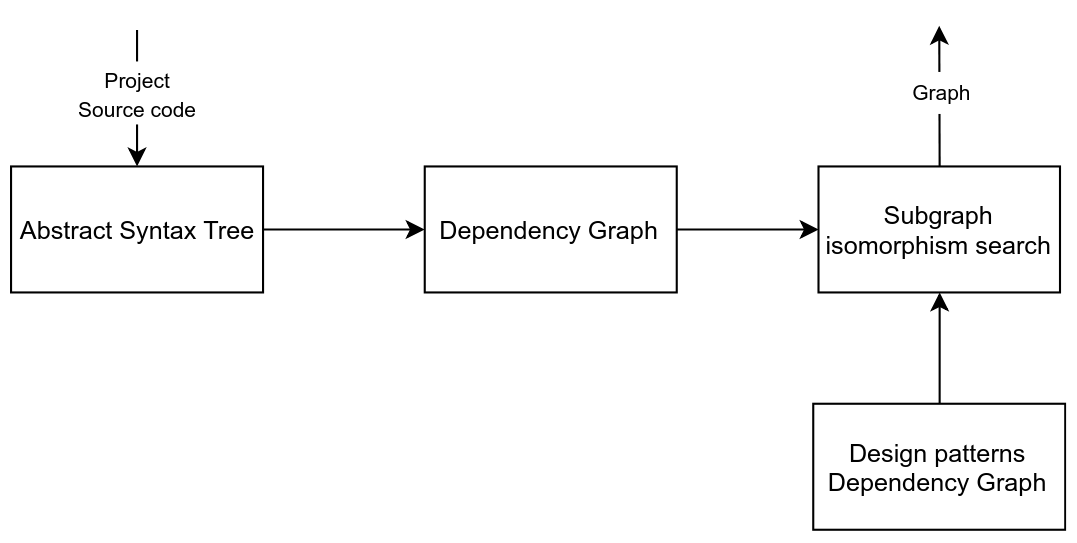
\includegraphics[scale=0.36]{images/general_architecture_3_1}
	\caption{Quá trình kiểm tra sự tuân thủ mẫu thiết kế của mã nguồn}
	\label{fig:general_architecture}
\end{figure}

\section{Tiền xử lý mã nguồn Java}
\subsection{Xây dựng cây cấu trúc}
Đối với phương pháp kiểm tra sự tuân thủ mẫu thiết kế mà khóa luận đề xuất. Cần có một kiểu dữ liệu tường minh và thể hiện được toàn bộ cấu trúc của mã nguồn, trong khi đó mã nguồn của dự án là phức tạp và chưa nhiều thông tin không được dùng tới. Nếu dùng trực tiếp mã sẽ gây khó khăn trong quá trình giải quyết bài toán và ảnh hưởng tới hiệu năng của của công cụ được xây dựng. Do đó cần tiến hành tiền xử lý mã nguồn, xây dựng một kiểu cấu trúc dữ liệu phù hợp. Cây cấu trúc được để xuất như là một kiểu cấu trúc dữ liệu phù hợp nhất thể hiện được toàn bộ cấu trúc của mã nguồn dự án.
\\
\\
\textbf{Định nghĩa: }(\textit{Cây cấu trúc} \cite{jcia}) Là một đồ thị liên thông với $T = (N,E)$ trong đó $N = \{n_1,n_2,n_3...n_k \}$ là tập các nút trên cây đại diện cho tệp, lớp, phương thức, biến... $E = \{(e_i,e_j) | e_i \in N , e_j \in N \}$ mỗi cặp $e_ie_j$ là cặp hai đỉnh kề của đồ thị.\\\\
Mô tả phương pháp tiền xử lý mã nguồn:
\begin{figure}[h]
	\centering
	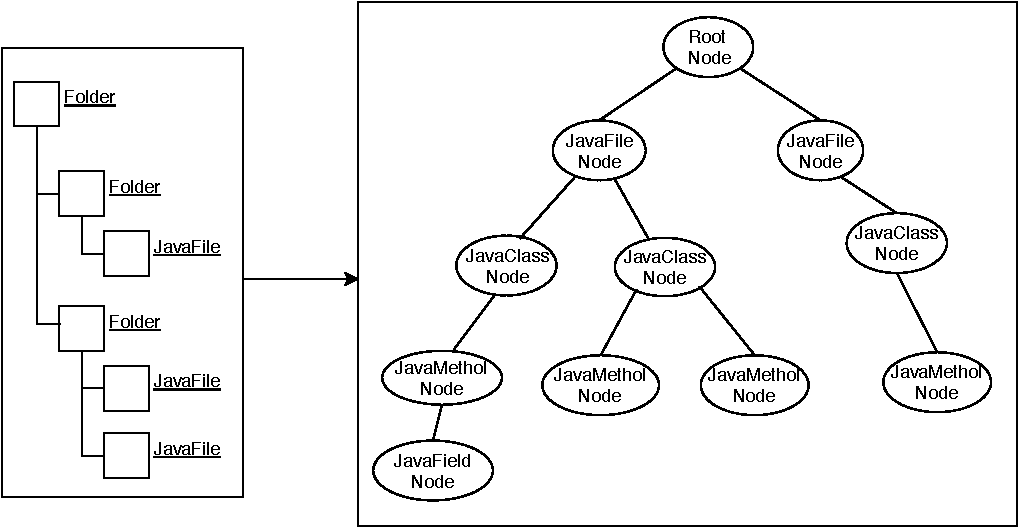
\includegraphics[scale=0.32]{images/structure_tree}
	\caption{Xây dựng cây cấu trúc từ mã nguồn}
	\label{fig:universe}
\end{figure}\\
Các nút trên cây được ánh xạ về bốn loại: tệp tin (\textit{Java}), lớp, phương thức và một loại nút thể hiện cho những định dạng còn lại. Mỗi loại nút của cây chứa những thuộc tính khác nhau và thông tin về nút cha, con của nó. Những thông tin trên mỗi nút được phân tích từ AST.
\subsection{Xác định thuộc tính cho mỗi nút trên cây cấu trúc}

Thành phần của một lớp gồm bốn phần chính: \textit{Class type, Class dependency, Class variables, Method }. Trong đó \textit{Class type} của một nút (class) thể hiện nút đó đóng vai trò như một:\textit{ Class, Abstract class, Template class} hay \textit{Interface}. \textit{Class depedency} ở đây  ta xét tới phụ thuộc thừa kế của lớp, phụ thuộc thừa kế bao gồm hai loại: kế thừa từ một class, kế thừa từ Interface. \textit{Method} là định nghĩa một hành vi của lớp, \textit{Method} bao gồm các thành phần: \textit{Local variable, Return type, Input paramater}  . \textit{Class variables} là biến của một lớp được khởi tạo bên ngoài các \textit{Method}. \textit{Local variable} là biến chỉ được khai báo và sử dụng trong phạm vi \textit{Method}. \textit{Return type} là kiểu dữ liệu mà phương thức sẽ trả về nếu \textit{Return type} là kiểu \textit{void} thì phương thức sẽ không trả về giá trị. \textit{Input paramter} xác định kiểu giá trị đầu vào cho phương thức.
\\
\begin{figure}[!htbp]
	\centering
	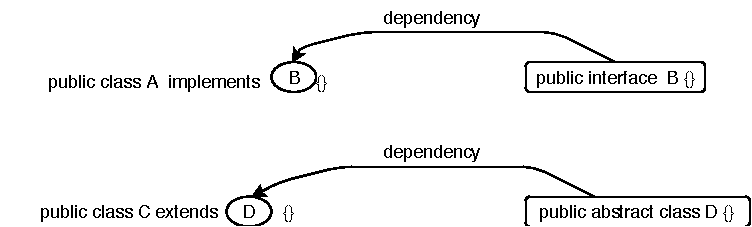
\includegraphics[scale=0.45]{images/class_dependency}
	\caption{Phụ thuộc thừa kế của lớp}
	\label{fig:dependecy_extend}
\end{figure}\\\\
Hình 3.3 mô tả hai loại phụ thuộc kế thừa. Trong đó A là một Class thừa kế từ B là một Interface qua phương thức extend, C là một class thừa kế D qua phương thức implement với D là một abstract class.\\\\
\begin{figure}[h]
	\centering
	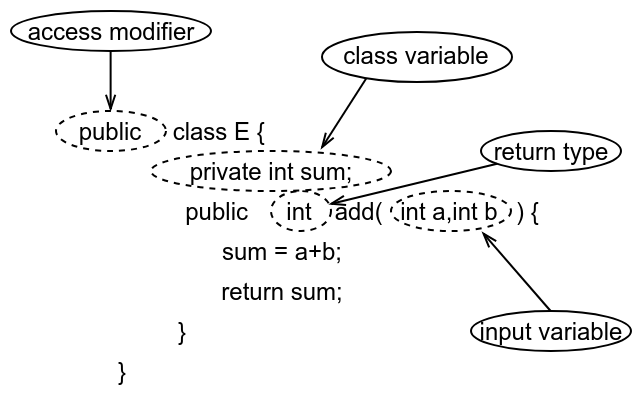
\includegraphics[scale=0.45]{images/class_method_structure}
	\caption{Các thành phần cơ bản trong class}
	\label{fig:class_structure}
\end{figure}\\
\noindent Hình 3.4 Các thành phần cơ bản của \textit{Class}. Trong đó E là một Class với Access modifer là public, Class variable là sum với kiểu giá trị int và Access modifier là private, Method add() có kiểu trả về là int và hai biến đầu vào là a và b.
\newpage
\noindent Bảng 3.1 mô tả đầy đủ những thông tin cần xác định cho mỗi loại nút trên cây cấu trúc, nhằm phục vụ cho việc phân tích cấu trúc mã nguồn và xây dựng đồ thị phụ thuộc sẽ được trình bài tại phần \textbf{3.2} và \textbf{3.3} của chương này.
\begin{table}[h]
	\centering
	\renewcommand{\arraystretch}{1.2}
	\begin{tabular}{|l|l|}
		\hline
		\textbf{Node} & \textbf{Popertiesoperties}                                        \\ \hline
		Class            & \begin{tabular}[c]{@{}l@{}}NameType\\ Access modifier\\ Extended Class\\ Implemented Class\\ Childrent Node: Field, Method\end{tabular} \\                                       \hline
		Method              & \begin{tabular}[c]{@{}l@{}}Name\\ NameReturn Type\\ Access modifier\\ Parameter\\ Body\end{tabular} \\ \hline
		Field               &\begin{tabular}[c]{@{}l@{}}Name\\ Value type\\ Access modifier\end{tabular} \\ \hline
	\end{tabular}
	\caption{Thuộc tính trên mỗi nút}
	\label{tbl:node_properties}
\end{table}\\


\noindent Việc trích xuất các thông tin từ mã nguồn cho các nút trên cây, được thực hiện thông qua AST. Với mỗi thành phần mã nguồn, ta sử dụng JP để sinh AST tương ứng với thành phần đó từ đó trích xuất các thuộc tính cần thiết cho mỗi nút trên cây cấu trúc.\\
Hình 3.5 mô tả một AST với một Class Java tương ứng. Trong đó một lớp Java được phân tách thành dạng cây với các nút gốc chứa các toán tử, các nút lá chứa các toán hạng. Ví dụ như return = 42, trong đó return là một toán tử ứng với 'ReturnStatement' và '42' là toán hạng ứng với nút lá.
\begin{figure}[!htbp]
	\centering
	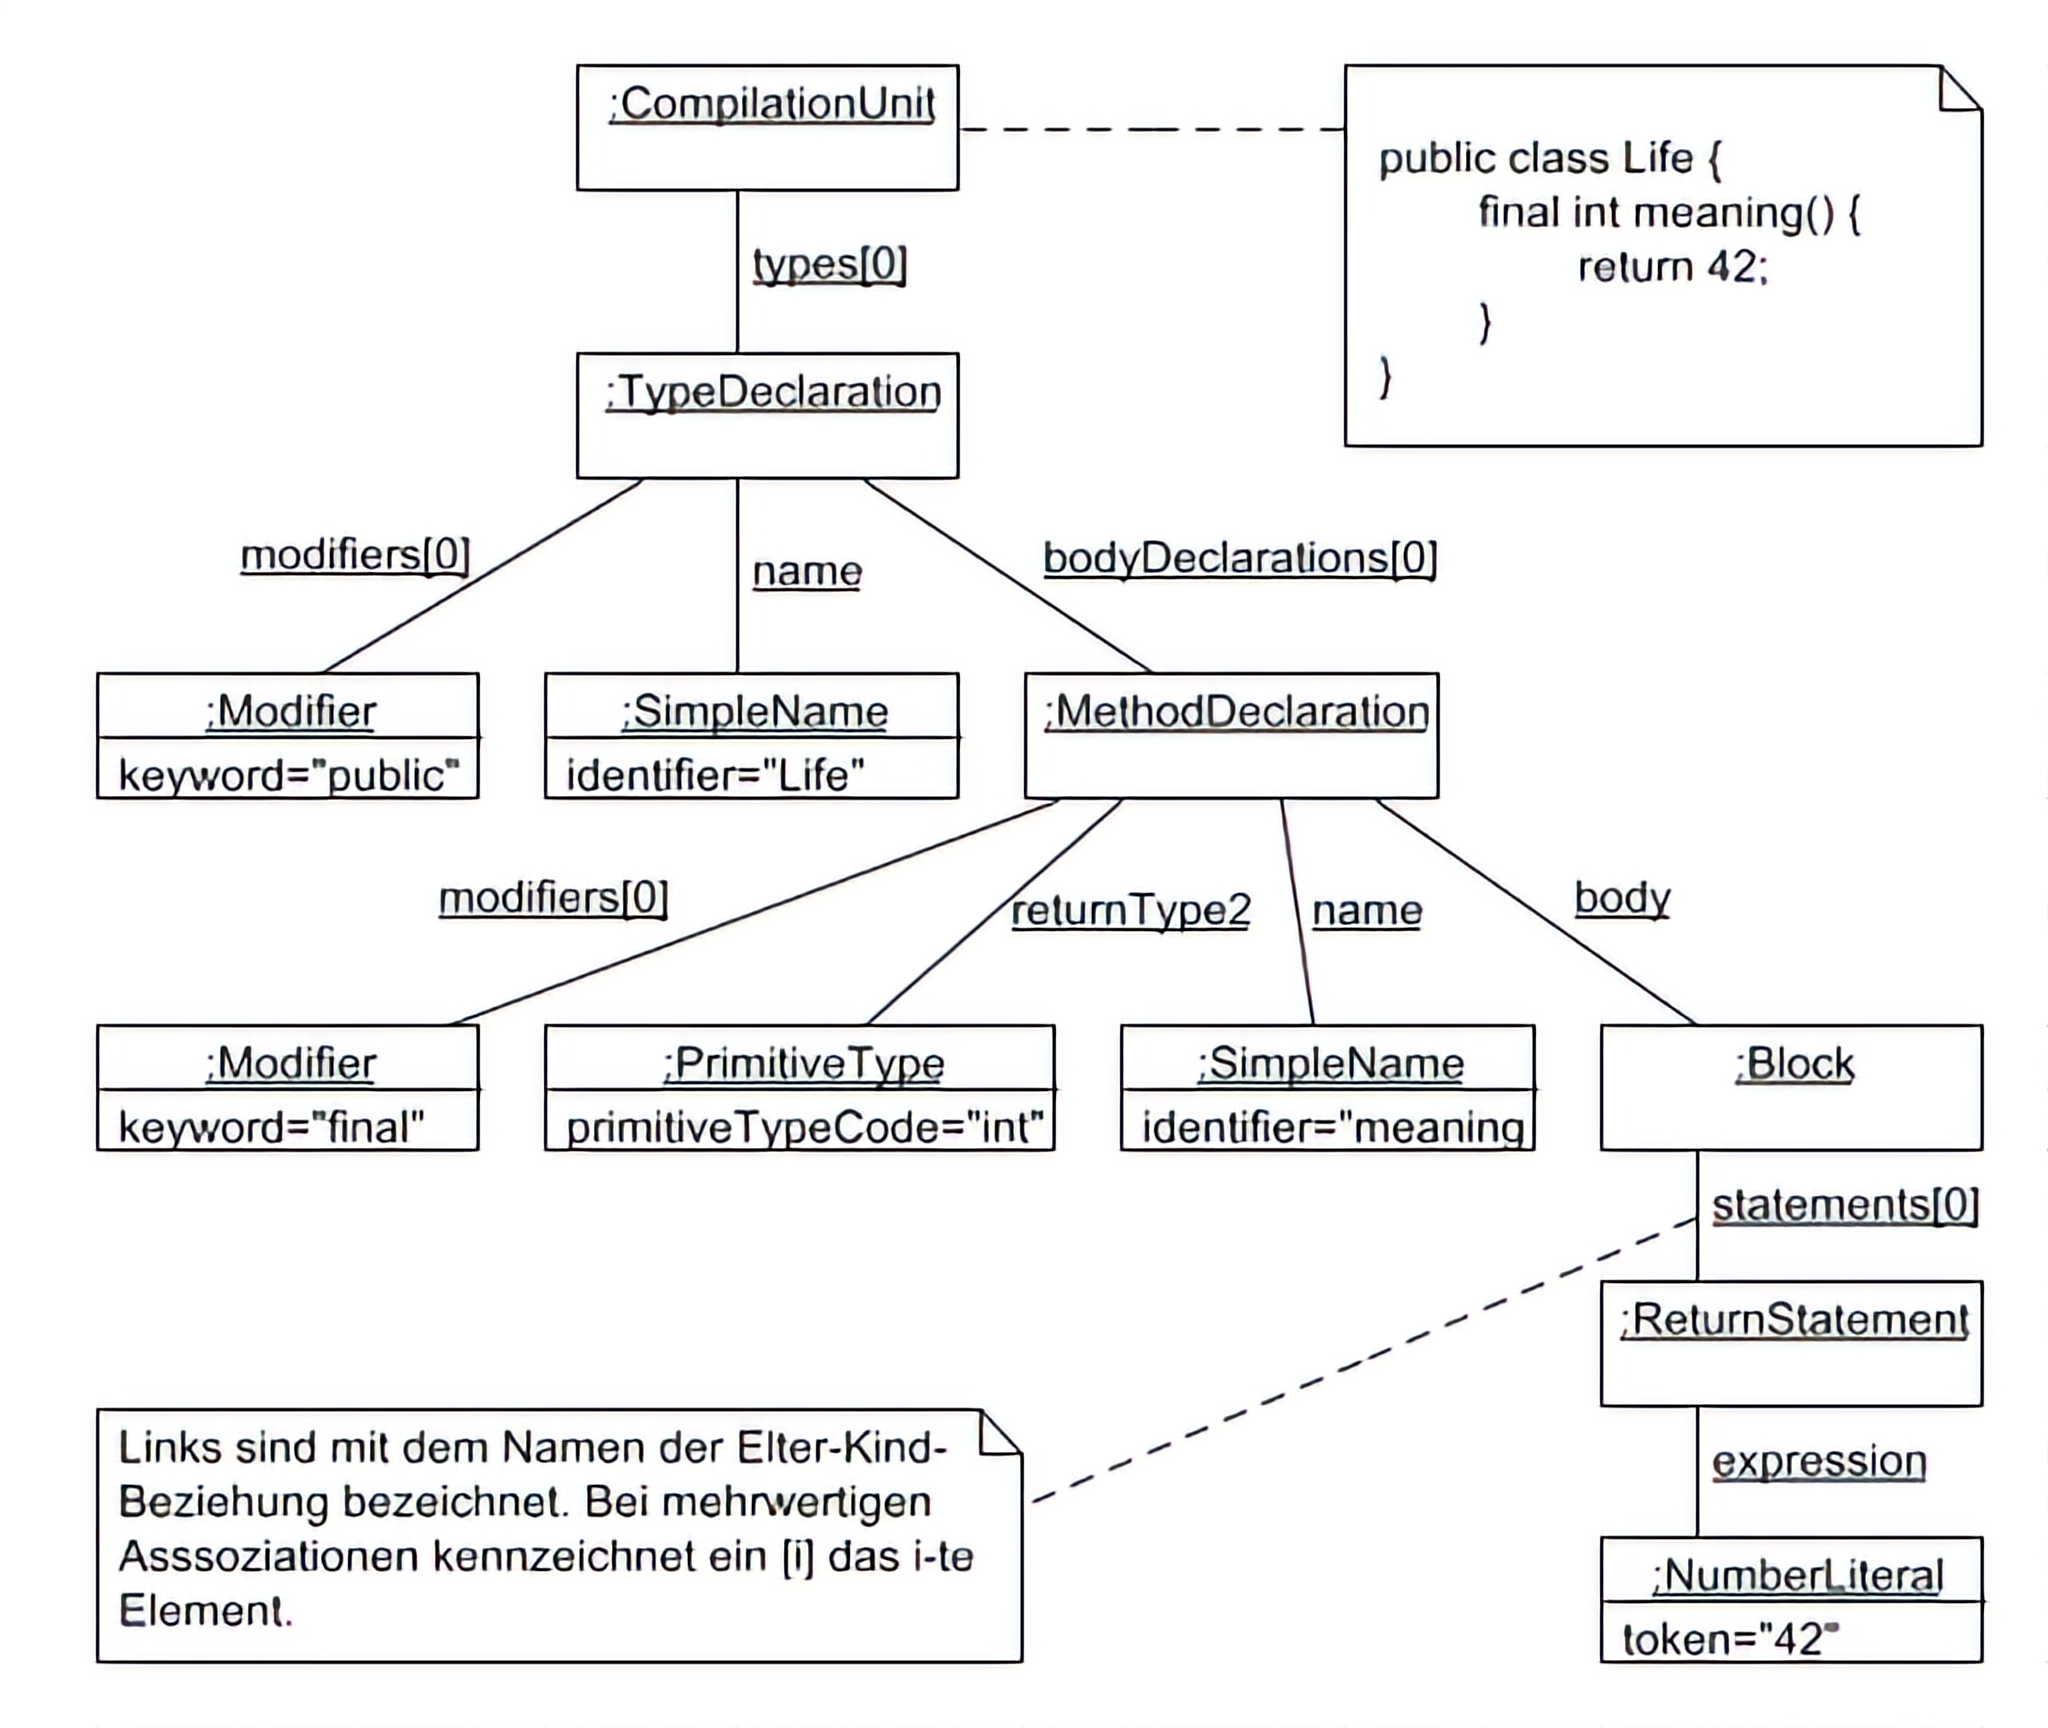
\includegraphics[scale=1]{images/ast_class_java-boring}
	\caption{Abstract syntax tree đối với Java class}
	\label{fig:ast_for_java_class}
\end{figure}
\section{Phân tích cấu trúc mã nguồn Java}
\indent Cấy cấu trúc thể hiện thể hiện chi tiết về cấu trúc của mã nguồn bao gồm các khía cạnh về tính hướng đối tượng bên trong mã nguồn. Phân tích cấu trúc mã nguồn nhằm xác định được những đặc điểm về mặt phụ thuộc giữa các thành phần mã nguồn được hình thành bới việc áp dụng những mẫu thiết kế bên trong mã nguồn. Xác định được những được những đặc nêu trên là tiền để để kiểm tra sự tuân thủ mẫu thiết kế bên trong mã nguồn.
\subsection{Phân tích phụ thuộc giữa các thành phần trong mã nguồn}
Đối với phương pháp mà khóa luận này đề xuất, việc phân tích phụ thuộc giữa các thành phân bên trong mã nguồn xoay quanh việc phân tích phụ thuộc giữa các lớp trong mã nguồn. Đối với loại phụ thuộc giữa các lớp trong mã nguồn Java bao gồm: Direct \& Indirect dependency, Polymorphism dependency, Inheritance Dependency, Use Dependecy,Behavior Dependency\\\\
\textbf{Polymorphism dependency}: Ở đây ta xem xét hai trường hợp của lọai pụụ thuộc này. Trường hợp thứ nhất khi một Class thừa kế một Interface bằng phương thức Implement. Ví dụ Class, A  thừa kế một interface B, Class A sẽ thừa kế những phương thức của Interface C, tức là tại Class A những phương thức được Interface C định nghĩa sẽ được triển khai. Ngoài ra tham chiếu của Interface B có thể trỏ tới đối tượng của Class A, trong trường hợp đó đối tượng tạo được trỏ tới bởi B chỉ có thể thực hiện những phương thức mà B đã định nghĩa, nhưng phương thúc khác của A sẽ bị làm mờ đi. Trường hợp thứ hai, phụ thuộc xảy ra khi một class thừa kế một class khác thông qua phương thức extends. Ví dụ, class C thừa thế class D, lúc này ta coi D như là Class cha, với C là class con, C sẽ thừa hưởng mọi thuộc tính và phương thức của  D, do đó C có thể ghi đè những phương thức của D, ngoài ra, tham chiếu của Class D có thể trỏ tới đối tượng của class C. Hình 3.6 và 3.7 mô tả ví dụ về hai trường hợp mà ta đã đề cập.
\begin{figure}[!htbp]
	\vspace*{-2cm}
	\centering
	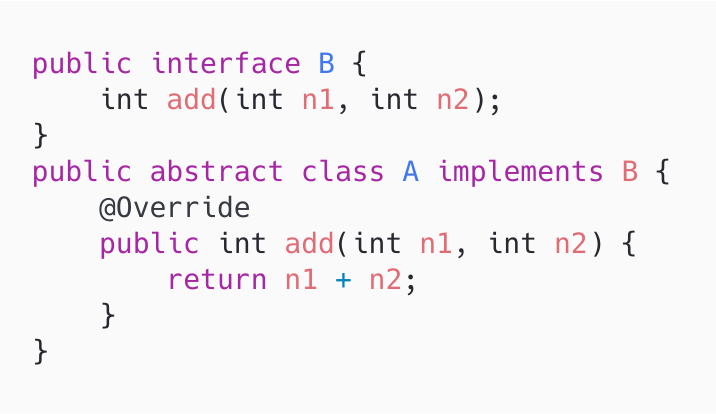
\includegraphics[scale=0.5]{images/AimplementsB}
	\caption{Mối quan hệ giữa một Class vớ một Interface qua phương thức Implements}
	\label{fig:A_implemets_B}
\end{figure}
\begin{figure}[!htbp]
	\centering
	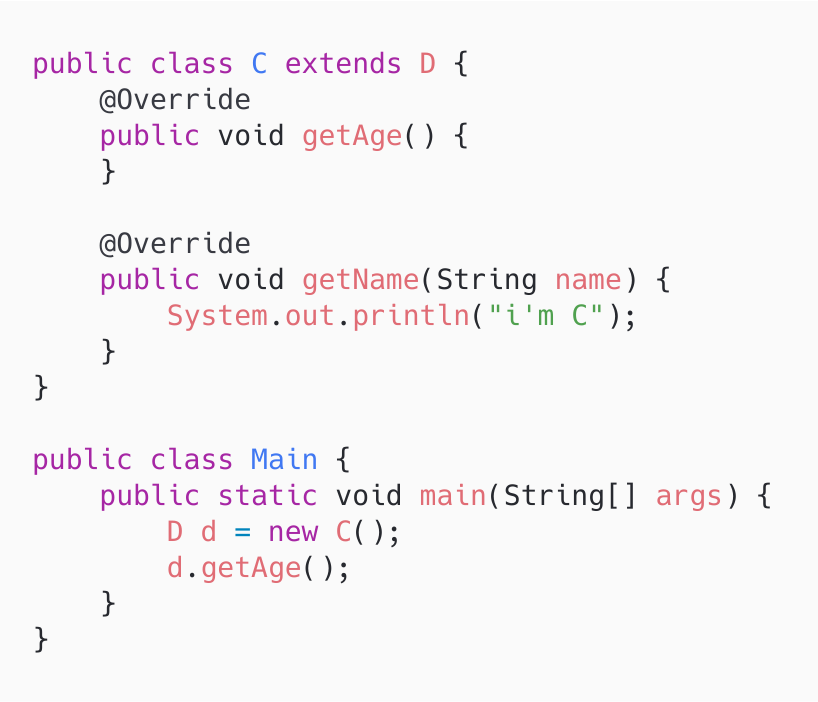
\includegraphics[scale=0.5]{images/CextendD}
	\caption{Mối quan hệ giữa một Class với một Class qua phương thức extends}
	\label{fig:CextendD}
\end{figure}



\pagebreak
\noindent \textbf{Inheritance Dependency}: Khi một Class có được các thuộc tính và phương thức của một Class khác. Những thuộc tính và phương thức này được quản lý theo thứ tự phân cấp từ lớp con tới lớp cha, việc xử lý phân cấp được quyết định trong quán trình chương trình đang thực thi bởi JVM. Ví dụ, ta có Class D thừa kế Class E với phương thức \textit{extends}, khi đó D sẽ thừa hưởng các phương thưc và thuộc tính của E. Trong trường hợp các phương thức và thuộc tính của D có \textit{Access modifier} là \textit{private}, khi đó đối tượng của Class A sẽ không thể gọi tới những thuộc tính, phương thức này. Hình 3.7 mô tả mối quan hệ thừa kết giữa hai Class Java.\\\\
\begin{figure}[!htbp]
	\centering
	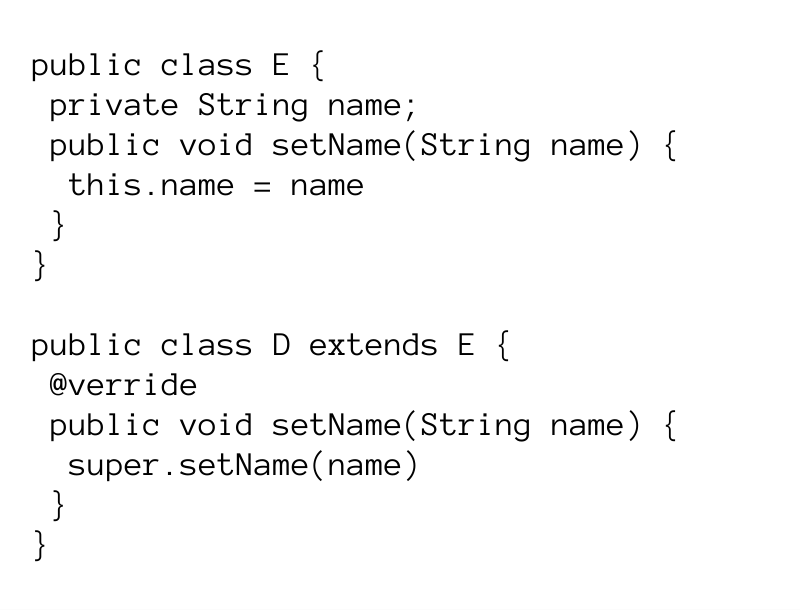
\includegraphics[scale=0.5]{images/D_extends_E}
	\caption{Mối quan hệ giữa một Class vớ một Interface qua phương thức Implements}
	\label{fig:D_extends_E}
\end{figure}\\\\
\textbf{Use Dependency}: Không giống với \textit{Inheritance Dependency} hay \textit{Polymorphism dependency}, Use Dependency thể hiện sự tương quan giữa các Class về mặt tương tác dữ liệu,khi các đối tượng của lớp này được sử dụng nhứ là thuộc tính, giá trị trả về, kiểu dữ liệu đầu vào, biến địa phương của phương thức của Class khác hoặc được sử dụng để khai kiểu cho một Generic Class.

\begin{figure}[!htbp]
	\centering
	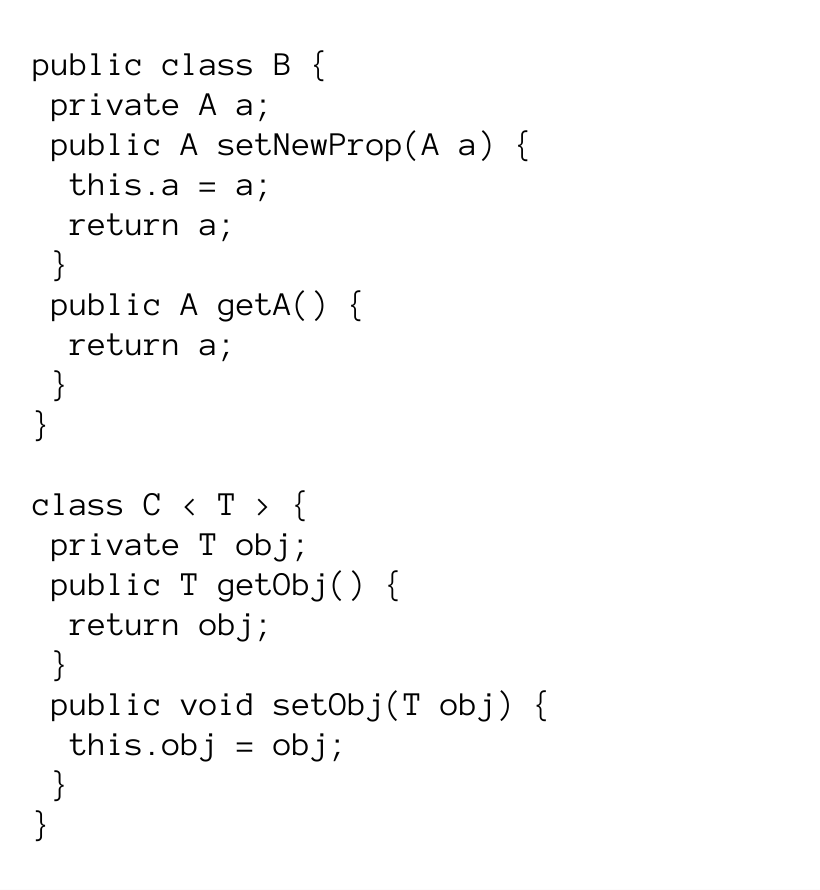
\includegraphics[scale=0.5]{images/use_dependency}
	\caption{Mô tả Use dependency}
	\label{fig:}
\end{figure}
\noindent Hình 3.8 mô tả \textit{Use dependency}. Chia làm hai ví dụ nhỏ. Ví dụ thứ nhất, đối tượng của Class A được khai báo là thuộc tính của Class B, những phương thức của Class B có kiểu trả về, kiểu dữ liệu đầu vào là đối tượng của Class A. Ví dụ thứ hai, Class C khai bảo kiểu Generic, và định nghĩa những phương thức sử dụng kiểu Generic, tức là kiểu dữ liệu mà Class định nghĩa cho các phương thức, thuộc tính của nó sẽ phụ thuộc vào kiểu dữ liệu được khai báo khi Class được sử dụng.
\\\\

\noindent \textbf{Behavior Dependency}: Phụ thuộc thể hiện hành vi của các dối tượng của mỗi Class, tức là sự tương tác của đối tượng của Class này với đối tượng của một Class khác. Điều kiện cần của loại phụ thuộc này đó là giữa Class có tồn tại Inheritance dependency.
\subsection{Xây dựng đồ thị phụ thuộc từ cây cấu trúc}
Đồ thị phụ thuộc nhằm thể hiện mối quan hệ về cấu trúc giữa các thành phần trong mã nguồn, sự tương tác giữa các thành phần như Class, Methol, Field.v.v với nhau bên trong mã nguồn, tạo nên sự ảnh hưởng qua lại giữa chúng
việc phân tích và xây dựng đồ thị phụ thuộc xoay quanh phương pháp kiểm sự tuân thủ mẫu thiết kế bên trong mã nguồn dự án.
Đối với phương pháp mà khóa luận này đề xuất, đồ thị phụ thuộc được xây dựng là đồ thị có hướng.\\\\
\noindent \textbf{Đồ thị phụ thuộc} (\textit{Định nghĩa}): là một đồ thị có hướng $G = \{V,E \}$, trong đo $V = \{v_1,v_2,v_3..v_k\}$ là tập các đỉnh của đồ thị với mỗi đỉnh tương ứng với một Class trong mã nguồn, $E = \{ e_ie_j | e_i \in V, e_j \in V  \}$ là tập các cạnh đinh hướng của đồ thị từ đỉnh $e_i$ tới $e_j$. Trên mỗi cạnh nối hai đỉnh chứa thuộc tính thể hiện sự phụ thuộc giữa hai đỉnh (class) của đồ thị (mã nguồn)\\

\noindent Từ việc phân tích các loại phụ thuộc phái trên, ta tiến hành định nghĩa một tập những phụ thuộc, được hiẻu như là các cạnh của đồ thị phụ thuộc. Tập các đỉnh là những Class. Được kiệt kê tất cả trong Bảng 3.2 \cite{orucc2016} và Bảng 3.3 \cite{orucc2016}

\begin{table}[!htbp]
	\centering
	\caption{Các loại đỉnh của đồ thị phụ thuộc}
	\label{tbl:java-class-type}
	\begin{tabular}{|p{3cm}|p{9cm}|}
		\hline
		\textbf{Kí hiệu} & \textbf{Loại} \\ \hline
		C				& Class\\ \hline
		I				& Interface \\ \hline
		A				& Abstract class \\ \hline
		T				& Template class \\ \hline         
	\end{tabular}
\end{table}

\begin{table}[!htbp]
	\centering
	\caption{Các loại phụ thuộc Java}
	\label{tbl:field-ct}
	\begin{tabular}{|l|l|}
		\hline
		\textbf{Kí hiệu} & \textbf{Ý nghĩa}                                        \\ \hline
		X               & class A extends class B                                        \\ \hline
		I               & class A implement class B                                                 \\
		\hline
		C               & class A create object of class B                                                \\
		\hline
		R              &  class A has the return type of class B             \\ \hline
		MC              & class A call a method of class B                          \\ \hline
		F              &  class A has the field type of class B   \\ \hline
		MR              &class A has a method with return type of class     \\ \hline
		MI              & \begin{tabular}[c]{@{}l@{}}class A has a method that has an input parameter\\ with the type of Class B \end{tabular} \\ \hline
		ML               & \begin{tabular}[c]{@{}l@{}}class A has a method that defines a local variable\\ with the type of class B\end{tabular} \\ \hline
		G              & class A uses class B in a generic type declaration   \\ \hline
		M               & class A has related with its method of class B \\ \hline
		O                &  class A overrides of class B \\  \hline
	\end{tabular}
\end{table}



\newpage
\noindent Để xây dựng đồ thị phụ thuộc ta duyệt lần lượt từng cặp nút (class) trên cây cấu trúc, với mỗi cặp ta kiểm tra xem cặp đó có tồn tại một trong nhữung loại phụ thuộc đã được được nghĩa hay không, nếu có tiến hành gắn phụ thuộc cho cặp nút đó.
\begin{thuattoan}
		\label{algo:dependency-analyze}
		\caption{$JavaDependencyAnalyze(Root)$}
		\SetKwInOut{Input}{Input}
		\SetKwInOut{Output}{Output}
		\Input{T là tập các nút trên cây cấu trúc}
		\Output{Graph là đồ thị phụ thuộc}
		$C$ = tập các nút lớp (Class Node) trên cây T \;
		$G$ = $New Grpah()$\;
		\ForEach{$c_i \in C$ , $C$ }{
			$d$ , $c_j$ = $analyzerClassLevel$($c_i$,$C$,$G$)\;
			
			\If{$d$ $not$ $empty$}{
					$new$ $Dependency$($c$,$c_j$,$d$)\;
			}
		
			
			$analyzerMethodLevel$($c_i$,$C$,$G$)\;
			\If{$d$ $not$ $empty$}{
				$new$ $Dependency$($c$,$c_j$,$d$)\;
			}
			
			$analyzerdFieldLevel$($c_i$,$C$,$G$)\;
			\If{$d$ $not$ $empty$}{
				$new$ $Dependency$($c$,$c_j$,$d$)\;
			}
		}
	
		\Return $G$\;
\end{thuattoan}

\newpage
\subsection{Ví dụ minh họa}
\begin{figure}[!htbp]
	\centering
	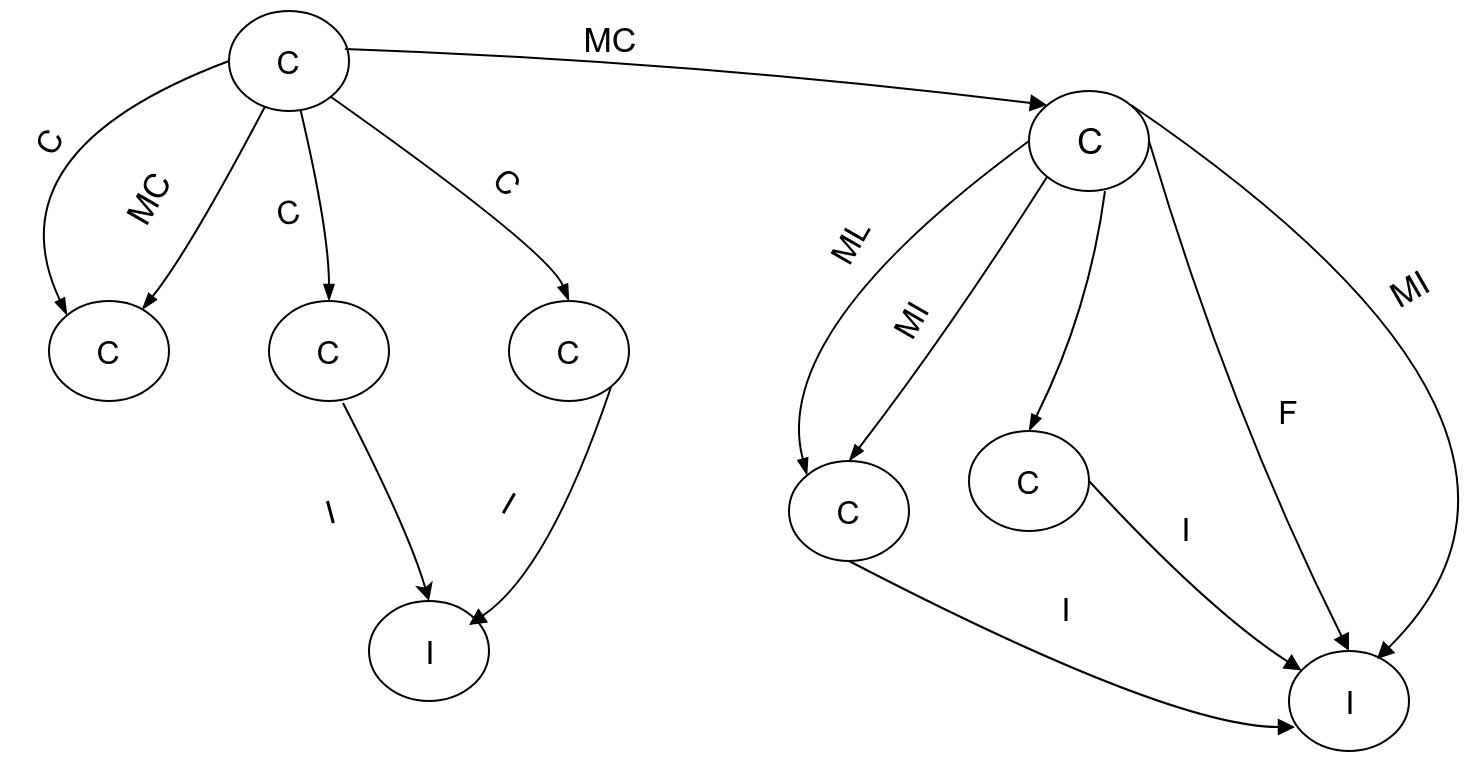
\includegraphics[scale=0.25]{images/example_graph_dependency}
	\caption{Ví dụ minh họa về đồ thị phụ thuộc}
	\label{fig:example_graph_dependency}
\end{figure}
\noindent Để hiểu rõ hơn về đồ thị phụ thuộc ta xem xét ví dụ Hình 3.10. Là độ thị phụ thuộc sinh ra từ một mã nguồn. Với các Class là các đỉnh của đồ thị, \textbf{C} tương ứng class và \textbf{I} tương ứng với Interface. Những class, interface này tương tác lẫn nhau qua những phụ thuộc như \textbf{MI} \textit{: class A has a method that has an input parameter with the type of Class B},...v.v\\
Đồ thị này là tiền đề đê kiểm tra sự tuân thủ mẫu thiết kế trong mã nguồn sẽ được trình bày ở phần sau đây.

\section{Kiểm tra sự tuân thủ mẫu thiết kế bên trong mã nguồn}
Quá trình kiểm tra sự tuân thủ mẫu thiết kế trong mã nguồn, tức là kiểm tra sự tồn tại của một mẫu thiết kế bên trong mã nguồn. Đầu vào củao phần này gồm hai thành phần. Thứ nhất, \textbf{đồ thị phụ thuộc} của mã nguồn dự án. Thứ hai, \textbf{đồ thị phụ thuộc} của những mẫu thiết kế. Ta sẽ đi tiến hành kiểm tra sự tồn tại của từng mẫu thiết kế bên trong mã nguồn. 
Đầu vào của bài toán sẽ là hai đồ thị có hướng. Bản chất của vấn đề sẽ là tìm kiếm sự tồn tại của một đồ thị bên trong một đồ thị khác. Đo đó, thuật toán tìm kiếm đồ thị đẳng cấu \textbf{VF2 algorithm for the Subgraph Isomorphism Problem} được đề xuất để giái quyết bài toán.

\noindent \textbf{Ý tưởng của giải thuật VF2} \cite{vf2}:
\begin{enumerate}
	\item Assume the problem is to find a subgraph in G1 isomorphic to the graph G2.
	\item The main idea is to construct a state S which contains a correct partial match between nodes of G1 and G2
	\item M(s) identifies two sub graphs of G1 and G2, say G1(s) and G2(s),
	 obtained by selecting from G1 and G2 only the nodes included in M(s),
	  and the branches connecting them. Where s is a state of the matching process. 
	\item The main problem is extending M(s) with new branches.
	\item An extension of S is adding a pair (n,m) where n belongs to G1 and m belongs to G2.
	\item Feasibility rules is a set of rules that are able to verify the consistency conditions,
	 making possible the generation of consistent states only.
\end{enumerate}
\newpage
Tập các luật (Feasibility Rules \cite{vf2_1368}) được định nghĩa cho giải thuật VF2 như sau:
\begin{figure}[!htbp]
	\centering
	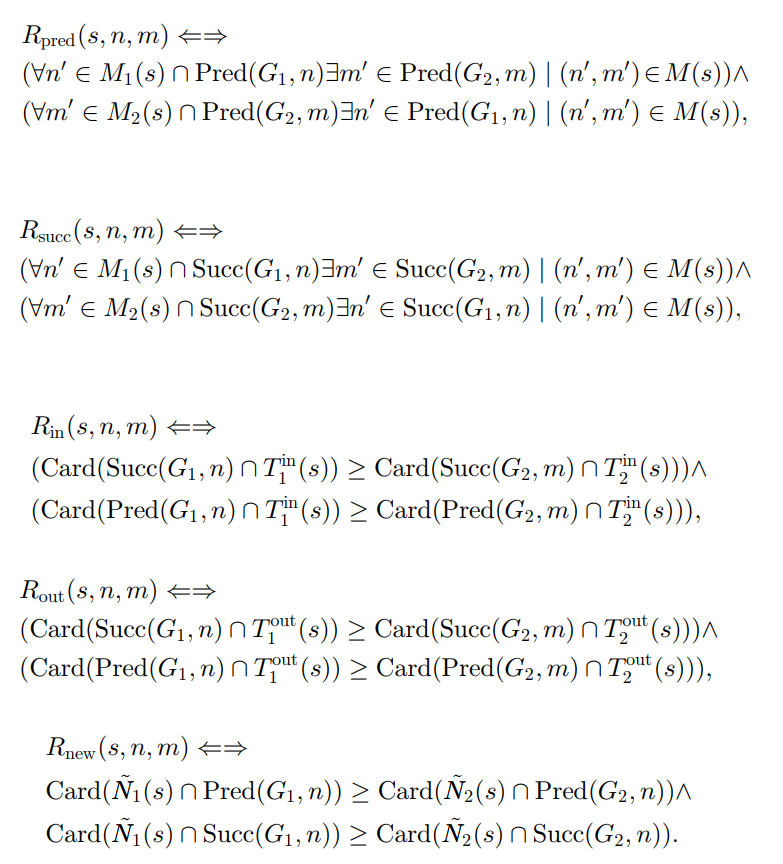
\includegraphics[scale=0.5]{images/rule_}
\end{figure}

\newpage
\noindent Chi tiết gỉai thuật VF \cite{vf2_1368}:
\begin{thuattoan}[!htbp]
	\label{algo:VF2}
	\caption{$VF2$}
	PROCEDURE Match(s)\\
	\SetKwInOut{Input}{Input}
	\SetKwInOut{Output}{Output}
	\hspace{5mm}\Input{an intermediate state $s$; the initial state $s_0$ has $M(s_0) = \emptyset $}
	\hspace{5mm}\Output{the mappings between the two graphs}
	\hspace{5mm}IF $M(s)$ covers all the node of G2\\
		\hspace{10mm} \Return M(s)
		
	\hspace{5mm}ELSE\\
		\hspace{10mm} Compute the set $P(s)$ of the paris candidate for inclusion in $M(s)$\\
		\hspace{10mm} FOREACH	$p \in P(s)$ \\
		\hspace{10mm} IF the feasibility reles successd for the inclusion of p in $M(s)$\\
				\hspace{20mm} Compute the state $s'$ obtained by adding p to $M(s)$\\
				\hspace{20mm} CALL Match($s'$)\\
			
		\hspace{15mm} END IF
		
		\hspace{10mm}END FOREACH\\
		\hspace{10mm}Restore data structures\\
	\hspace{5mm}END IF\\
	END PROCEDURE Match
\end{thuattoan}

\begin{thebibliography}{9}
	\section*{Tiếng Việt}
	\section*{Tiếng Anh}
	\bibitem{orucc2016}
	 Murat Oruc, Fuat Akal, Hayri Server. Detecting Design Patterns in  Object-Oriented Design Models By Using Graph Mining Approach. pp 115,2016
	
	\bibitem{jcia}
	Ba Cuong Le, Son Nguyen Van, Duc Anh Nguyen, Ngoc Hung Pham, Hieu Vo Dinh. JCIA: A Tool for Change Impact Analysis of Java EE Applications. Information Systems Design and Intelligent Applications, pp.105-114, 2018.
	
	\bibitem{jp}
	Nicholas Smith, Danny van Bruggen, Federico Tomassetti
	JavaParser: Visited
	Analyse, transform and generate your Java code base
	
	\bibitem{vf2}
	Luigi P. Cordella, Pasquale Foggia, Carlo Sansone,and Mario Vento. A (Sub)Graph Isomorphism Algorithm for
	Matching Large Graphs 10-2004 P1367
	
		\bibitem{vf2_1368}
	Luigi P. Cordella, Pasquale Foggia, Carlo Sansone,and Mario Vento. A (Sub)Graph Isomorphism Algorithm for
	Matching Large Graphs 10-2004 P1368-1369
\end{thebibliography}
\end{document}
